%%%%%%%%%%%%%%%%%%%%%%%%%%%%%%%%%%%%%%%%%%%%%%%%%%%%%%%%%%%%%%%%%%%%%%%%%%%%%%%%%%%%
% Document data
%%%%%%%%%%%%%%%%%%%%%%%%%%%%%%%%%%%%%%%%%%%%%%%%%%%%%%%%%%%%%%%%%%%%%%%%%%%%%%%%%%%%
\documentclass[12pt]{article} %report allows for chapters
%%%%%%%%%%%%%%%%%%%%%%%%%%%%%%%%%%%%%%%%%%%%%%%%%%%%%%%%%%%%%%%%%%%%%%%%%%%%%%%%%%%%
\usepackage{preamble}
\usepackage{caption,subcaption}
\newcommand{\vecx}{\boldsymbol{\vec{x}}}
\newcommand{\vecxdot}{\boldsymbol{\dot{\vec{x}}}}
\usepackage{cleveref}
\begin{document}

\begin{center}
   \textsc{\large MATH 272, Homework 5, \emph{Solutions}.}
\end{center}
\vspace{.5cm}

\begin{problem}
Let $\vecfieldV$ be a vector field in the plane $\R^2$ defined by
\[
\vecfieldV(x,y) = \begin{pmatrix} \frac{1}{2}x-y \\ x + \frac{1}{2}y \end{pmatrix},
\]
and let $\vecx(t) = \begin{pmatrix}  e^{\frac{1}{2}t} (-c_1 \sin(t) + c_2 \cos(t) ) \\ e^{\frac{1}{2}t} (c_1 \cos(t) + c_2 \sin(t)) \end{pmatrix}$ for $t\in [0,\pi]$ where $c_1$ and $c_2$ are yet undetermined constants.
\begin{enumerate}[(a)]
    \item Show that a flow of $\vecfieldV$ yields a linear system of equations.
    \item Show that $\vecx(t)$ is a flow of the vector field $\vecfieldV$.
    \item Let $\vecx(0)=\begin{pmatrix} 1 \\ 0 \end{pmatrix}$. Determine the particular solution to the initial value problem.
    \item \textbf{[MATLAB]} Plot the $\vecfieldV$ and your particular solution $\vecx$ simultaneously by modifying 
\begin{verbatim} vector_field_2d.m \end{verbatim}
 and
 \begin{verbatim} curve.m \end{verbatim} 
Then enter the following into the command window
\begin{verbatim} vector_field_2d \end{verbatim}
 followed by 
\begin{verbatim} curve \end{verbatim}
and finally to get the correct view enter
\begin{verbatim} view(0,90) \end{verbatim}
Choose good bounds for your plot so that the whole curve is visible.
\end{enumerate}
\end{problem}
\begin{solution}~
\begin{enumerate}[(a)]
    \item A flow of $\vecfieldV$ is given by
    \[
    \vecxdot(t) = \vecfieldV(\vecx)
    \]
    whereas a linear system of equations assumes the form
    \[
    \vecxdot(t) = [A(t)] \vecx,
    \]
    so we should attempt to find a $2\times 2$ matrix $[A(t)]$. Take
    \[
    [A(t)] = \begin{pmatrix} a_{11}(t) & a_{12}(t) \\ a_{21}(t) & a_{22}(t) \end{pmatrix},
    \]
    then
    \[
[A(t)] \vecx = \begin{pmatrix} a_{11}(t) x(t) + a_{12}(t) x(t) \\ a_{21}(t) x(t) + a_{22}(t) x(t) \end{pmatrix}.   
    \]
Thus, we can take 
\begin{align*}
a_{11}(t) &= \frac{1}{2} \\
a_{12}(t) &= -1 \\
a_{21}(t) &= 1\\
a_{22}(t) &= \frac{1}{2}.
\end{align*}
Thus, a flow defined by $\vecfieldV$ is linear.

\item We have
\[
\vecxdot = \begin{pmatrix} -e^{\frac{1}{2} t}\left( \left(\frac{1}{2} c_1 + c_2\right) \sin(t) + \left(c_1-\frac{1}{2}c_2\right) \cos(t)\right) \\ e^{\frac{1}{2} t}\left( \left(-c_1 +\frac{1}{2} c_2\right) \sin(t) + \left(\frac{1}{2}c_1+c_2\right) \cos(t)\right) \end{pmatrix}
\]
and likewise
\[
\vecfieldV(\vecx) = \begin{pmatrix} -e^{\frac{1}{2} t}\left( \left(\frac{1}{2} c_1 + c_2\right) \sin(t) + \left(c_1-\frac{1}{2}c_2\right) \cos(t)\right) \\ e^{\frac{1}{2} t}\left( \left(-c_1 +\frac{1}{2} c_2\right) \sin(t) + \left(\frac{1}{2}c_1+c_2\right) \cos(t)\right) \end{pmatrix}.
\]
Thus, $\vecx$ is a flow of $\vecfieldV$.

\item We have
\[
\begin{pmatrix} 1 \\ 0 \end{pmatrix} = \vecx(0) = \begin{pmatrix} c_2 \\ c_1 \end{pmatrix}.
\]
Thus, $c_1=0$ and $c_2=1$ and we have
\[
\vecx(t) = \begin{pmatrix} e^{\frac{1}{t}} \cos(t) \\ e^{\frac{1}{t}} \sin(t) \end{pmatrix}.
\]

\item Finally, we can plot this particular solution $\vecx$ overlayed on the vector field $\vecfieldV$.
\begin{figure}[H]
    \centering
    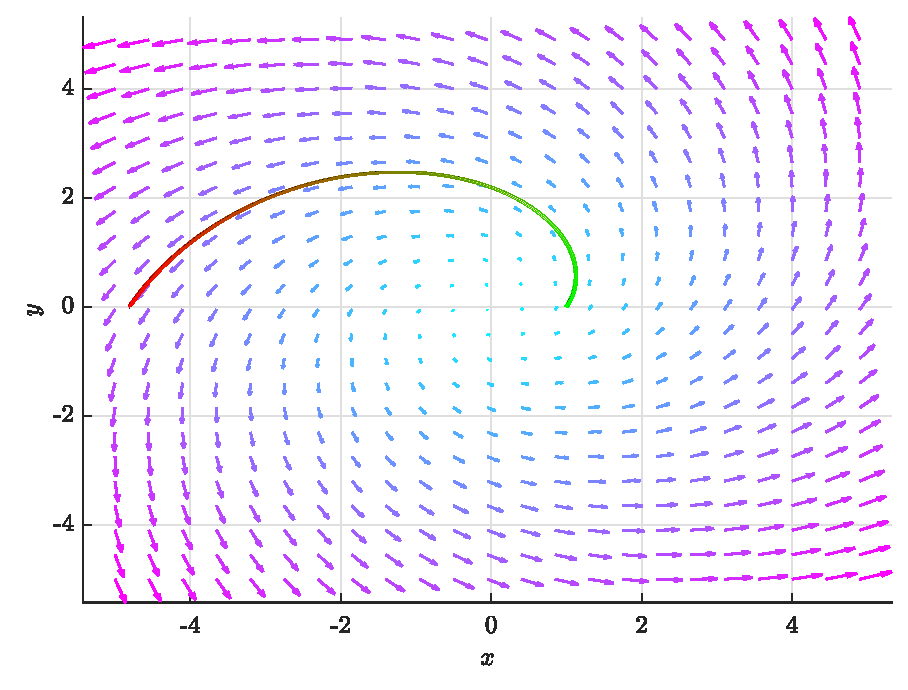
\includegraphics[width=.6\textwidth]{figures/flow}   
\end{figure}
\end{enumerate}
\end{solution}

\newpage

\begin{problem}
Let us consider the discrete heat equation for $n$ equally spaced particles on a line segment for which we have the following picture
\begin{figure}[H]
	\centering
	\resizebox{.9\columnwidth}{!}{\input{figures/equally_spaced_line_points.pdf_tex}}
\end{figure}
Let $u_j(t) \coloneqq u(x_j,t)$ denote the temperature of particle $j$ at time $t$, let $k_j$ be the thermal transport coefficient between particles $j$ and $j+1$, and let $f_j(t)=f(x_j,t)$ be the thermal energy source on particle $j$.
\begin{enumerate}[(a)]
    \item For the boundary particles $x_1$ and $x_n$, we have
    \[
    \dot{u}_1 = -k_1 u_1 + k_1 u_{2} + f_1 \qquad \textrm{and} \qquad \dot{u}_n = -k_n u_{n} + k_{n-1} u_{n-1} +f_n,
    \]
    which correspond to \emph{Neumann type boundary conditions}. Explain each term in the above equations.
    \item If we attached $x_1$ to $x_n$ with a material with a thermal transport coefficent of $k_0$ the above equations would need modification. Write these new equations. These are the \emph{periodic boundary conditions}. 
    \item Explain why periodic boundary conditions are the same as working with a circular domain.
    \item If we force $u_1$ and $u_n$ to be constant, what will the equations for the boundary particles be? These would be the \emph{Dirichlet type boundary conditions}.
    \item For the interior particles, we have the relationship
    \[
    \dot{u}_j = -k_{j-1}u_j - k_{j} u_j + k_{j-1}u_{j-1} + k_{j} u_{j+1} +f_j \qquad \textrm{for $j=2,\dots,n-1$}.
    \]
    Explain what each term describes in the above equation.
    \item In the limit as $n\to \infty$, we then have that $k$ is described as a function of position, $x$. The source free heat equation then reads
    \[
    \frac{\partial}{\partial t}u(x,t) = \frac{\partial}{\partial x} \left( k(x)\frac{\partial}{\partial x} u(x,t) \right) + f(x,t).
    \]
    Explain how this equation differs from the equation
    \[
    \frac{\partial}{\partial t}u(x,t) = k(x) \frac{\partial^2}{\partial x^2} u(x,t)+f(x,t).
    \]
\end{enumerate}
\end{problem}
\begin{solution}~
\begin{enumerate}[(a)]
    \item Let us concentrate on the two terms that appear in the first equation
    \[
\dot{u}_1 = \underbrace{-k_1 u_1}_{1} \underbrace{+ k_1 u_{2}}_{2}\underbrace{+f_1}_5.
    \]
    The rate of change of the temperature of particle 1, $\dot{u}_1$, depends on these three terms. For term 1, this corresponds to thermal energy leaving particle 1 at a rate given by the thermal transport coefficient $k_1$ and proportional to the temperature of particle $1$, $u_1$. Term 2 is the thermal energy entering particle 1 given by particle 2 at a rate $k_1$ proportional to the temperature of particle 2, $u_2$. The rates here are all the same since the two particles are connected by the same media. Thus, the rate of change of particle 1 can also be written as
    \[
    \dot{u}_1 = k_1(u_2-u_1) +f_1,
    \]
    which is equivalent to Newton's law of cooling with an additional heat source due to $f_1$. That is, the rate of change of temperature of a body is proportional to the difference of the temperature of the body and its surroundings in the case where the source term $f_1=0$. Term 3, $+f_1$, describes the rate of heat energy being added to particle 1. The equation for particle $n$ is completely analogous.

    \item The equations we have will need an additional term that corresponds to thermal transport to the particle at the other end of the interval. The original terms remain. Thus, we would have
    \[
\dot{u}_1 = -k_1 u_1 + k_1 u_{2} -k_0 u_1  + k_0 u_n+ f_1 \qquad \textrm{and} \qquad \dot{u}_n = -k_n u_{n} + k_1 u_{n-1} - k_0 u_n + k_0u_1 f_n.
    \]
    
    \item The above equations go to show that we have added medium between particles 1 and 2 so that 1 and 2 are in thermal contact. Thus, it is sensible to realize that we have taken this line of particles and attached endpoints to form a circle.

    \item The equations in this case are quite simple. We have
    \[
    \dot{u}_1 = 0 \qquad \textrm{and} \qquad \dot{u}_n = 0.
    \]
    Hence, we must also require that $f_1=0$ and $f_n=0$.
    

    \item Let us isolate the terms in the equation
\[
\dot{u}_j = \underbrace{-k_{j-1}u_j}_1 \underbrace{- k_{j} u_j}_2 \underbrace{+ k_{j-1}u_{j-1}}_3 \underbrace{+ k_{j} u_{j+1}}_4 \underbrace{+ f_j}_5.
\]
Terms 1 and 2 are negative, which mean they correspond to thermal energy lost by particle $j$. Indeed, thermal energy will be transported to particle $j-1$ through the medium with the thermal transport coefficient $k_{j-1}$ and proportional to $u_{j}$ (term 1) and thermal energy will transport to particle $j+1$ via the media with $k_j$ and proportional to $u_j$ (term 2). Terms 3 and 4 are positive, so they correspond to thermal energy gained by particle $j$. Particle $j$ receives thermal energy from particle $j-1$ via $k_{j-1}u_{j-1}$ and from particle $j+1$ via $k_j u_{j+1}$. Finally, term 5 is again the rate of thermal energy being added to particle $j$.

\item In the first equation, we have a product rule to apply to yield
\[
\frac{\partial}{\partial x} \left( k(x)\frac{\partial}{\partial x} u(x,t) \right) = \frac{d k}{dx} \frac{\partial u}{\partial x} + k \frac{\partial^2 u}{\partial x^2}.
\]
Indeed, this means that there is an extra term when we compare to the second equation. This term deals with the fact that the thermal transport medium itself can vary from point to point, and the gradient of this adds additional changes the diffusion process.
\end{enumerate}
\end{solution}

\newpage

\begin{problem}
    Consider the 1-dimensional homogeneous Laplace equation given by 
    \[
    \frac{\partial^2}{\partial x^2} u_E(x) = 0,
    \]
    with the domain $\Omega$ as the unit interval on the $x$-axis.  Take the Dirichlet boundary conditions $u_E(0)=T_0$ and $u_E(L)=T_L$.  Think of these values as the ambient temperature at the endpoints of the rod.  These temperatures are constant since the ambient environment is so large.
    \begin{enumerate}[(a)]
        \item Find the particular solution to this Laplace equation.
        \item Suppose that $v(x,t)$ is a solution to the 1-dimensional source free isotropic heat equation with zero Dirichlet boundary values. Show that 
        \[
        u(x,t)=v(x,t)+u_E(x),
        \]  
        is a solution to the 1-dimensional source free isotropic heat equation with Dirichlet boundary values $u(0,t)=T_0$ and $u(L,t)=T_L$.
        \item From Problem 1, we know that $\lim_{t\to \infty} v(x,t) = 0$.  Hence, show that the long time limit of a solution to the source free heat equation yields a solution to the Laplace equation.
        \item Argue why the equilibrium temperature profile of a rod can be found without solving the heat equation.
    \end{enumerate}
\end{problem}
\begin{solution}~
\begin{enumerate}[(a)]
    \item Note that we can integrate this equation twice to get a general solution
    \[
    u_E(x) = ax+b.
    \]
    Now, by matching boundary conditions, we have
    \[
    T_0=u_E(0) = b,
    \]
    so $b=T_0$. The other condition gives
    \[
    T_L = u_E(L) = aL+T_0,
    \]
    thus we have $a= \frac{T_L-T_0}{L}$. This means our particular solution is
    \[
    \boxed{    u_E(L) = \frac{T_L-T_0}{L}x - T_0.}
    \]
    
    \item First, we need to see if $u=v+u_E$ is a solution to the PDE.  If we plug this in, we have
    \begin{align*}
    \left( -k\frac{\partial^2}{\partial x^2} + \frac{\partial}{\partial t} \right) u &= \left( -k\frac{\partial^2}{\partial x^2} + \frac{\partial}{\partial t} \right)(v+u_E)\\
    &= \left( -k\frac{\partial^2}{\partial x^2} + \frac{\partial}{\partial t} \right)v(x,t) + \left( -k\frac{\partial^2}{\partial x^2} + \frac{\partial}{\partial t} \right)u_E(x).
    \end{align*}
    Now, note that
    \[
    \left( -k\frac{\partial^2}{\partial x^2} + \frac{\partial}{\partial t} \right)v(x,t) = 0,
    \]
    since we stated $v$ is a solution to this equation and note
    \[
    \left( -k\frac{\partial^2}{\partial x^2} + \frac{\partial}{\partial t} \right)u_E(x) = 0
    \]
    since $u_E(x)$ doesn't depend on $t$ and $u_E(x)$ solves the Laplace equation.
    
    Finally, we need to show that $u=v+u_E$ satisfies the boundary conditions.  Since $v(0,t)=0=v(L,t)$ by our supposition, we have that $u(0,t)=u_E(0)=T_0$ and $u(L,t)=u_E(L)=T_L$. Thus $u(x,t)$ is indeed a solution to the boundary value problem.
    
    \item We can take
    \[
    \lim_{t\to \infty} u(x,t) = \lim_{t\to \infty} \left( v(x,t) + u_E(x) \right) = u_E(x),
    \]
    which shows that $u_E(x)$ is the equilibrium temperature profile.  This is also the solution to the Laplace equation!
    
    \item To find the equilibrium temperature profile, we just needed to solve the Laplace equation.  That was the argument we made in (c). The equilibrium does not depend on time, since it is the result of waiting for $t\to \infty$. So, determining this is a completely separate problem if we wish it to be!
\end{enumerate}
\end{solution}

\newpage
\begin{problem}
    Using intuition from the previous problem, explain how one could solve the heat equation with a nonzero source term that only depends on $x$. In other words, how could one try to solve
    \begin{equation}
    \label{eq:poisson}
    \left( -k \frac{\partial^2}{\partial x^2} + \frac{\partial}{\partial t} \right) u(x,t) = f(x),
    \end{equation}
\end{problem}
\begin{solution}
One could argue that the equilibrium solution $u_E(x)$ will solve the equation
\[
-k\frac{\partial^2}{\partial x^2} u_E(x) = f(x),
\]
since this mimics what we did in the earlier problem.  This shows that when there are sources of heat in the material, they will contribute to the equilibrium temperature profile. How so? Take $u(x,t)=v(x,t)+u_E(x)$ as before, then
\begin{align*}
\left( -k \frac{\partial^2}{\partial x^2} + \frac{\partial}{\partial t} \right) u(x,t) &= f(x)\\
\left( -k \frac{\partial^2}{\partial x^2} + \frac{\partial}{\partial t} \right)( v(x,t)+u_E(x)) &= f(x)\\
\left( -k \frac{\partial^2}{\partial x^2} + \frac{\partial}{\partial t} \right) v(x,t) + -k \frac{\partial^2}{\partial x^2} u_E(x) &= f(x),
\end{align*}
and since $v(x,t)$ solves the 1d heat equation, are left with the above equation (\cref{eq:poisson}). Moreover, one should note that the boundary conditions must be handled by $u_E(x)$ as in problem 3.
\end{solution}

\newpage

\begin{problem}
    Consider the 2-dimensional source free isotropic heat equation given by
    \[
    \left( -k \Delta + \frac{\partial}{\partial t} \right) u(x,y,t) = 0,
    \]
    with the domain $\Omega$ as the unit square in the $xy$-plane. Take as well the Dirichlet boundary conditions $u(x,y,t)=0$ for $x$ and $y$ on the boundary of $\Omega$.
    \begin{enumerate}[(a)]
        \item Show that $u_{mn}(x,y,t)=\sin(m\pi x)\sin(n\pi y)e^{-k(n^2+m^2)\pi^2 t}$ is a solution to the PDE and Dirichlet boundary conditions for any non-negative integers $m$ and $n$.
        \item Show that a linear combination of solutions $u_{mn}$ and $u_{pq}$ is also a solution.
        \item For $m=n=1$ and $k=1$, plot the solution for the values $t=0$, $t=0.01$, $t=0.1$ and $t=1$.  Explain what is physically happening as time moves forward.
        \item Explain what varying the value for the conductivity $k$ does to the solution.  Feel free to use plots to support your hypothesis.
        \item Explain the mathematical reason why increasing $m$ and $n$ causes the solution to converge to zero more quickly.
        \item Explain the physical reason why increasing $m$ and $n$ causes the solution to converge to zero more quickly. Plots may help support your reasoning.
    \end{enumerate}
\end{problem}
\begin{solution}~
\begin{enumerate}[(a)]
    \item We can simply take the necessary derivatives to show that $u_{mn}$ is a solution.  We have
    \begin{align*}
    -k\Delta u_{mn} &= -ke^{-k(m^2+n^2)\pi^2 t} \left( -m^2\pi^2 \sin(m\pi x)\sin(n\pi y)-n^2\pi^2 \sin(m\pi x)\sin(n\pi y)\right) \\
    &=k(m^2+n^2)\pi^2 u_{mn}
    \end{align*}
    Then we also have
    \[
    \frac{\partial}{\partial t} u_{mn} = -k(m^2+n^2)\pi^2 u_{mn}.
    \]
    Hence, if we add these two together we have
    \[
    -k\Delta u_mn + \frac{\partial}{\partial t} u_{mn} = 0.
    \]
    So $u_{mn}(x,y,t)$ is a solution to the PDE for all $m$ and $n$.
    
    Now, as far as the boundary conditions go, the boundary to $\Omega$ is broken into four pieces
    \begin{align*}
    x\in [0,1] ~\& ~ y=0\\
    x\in [0,1] ~\& ~ y=1\\
    y\in [0,1] ~\& ~ x=0\\
    y \in [0,1] ~\& ~ x=1.
    \end{align*}
    Note that when $x=0$ or $x=1$, we have $\sin(m\pi x)=0$ since $m$ is an integer. Similarly we have for $y=0$ or $y=1$ that $\sin(n\pi y)=0$.  Thus, $u_{mn}=0$ along the boundary.
    
    \item Take $u=\alpha_{mn}u_{mn}+\alpha_{pq}u_{pq}$.  Then
    \begin{align*}
        \left( -k \Delta + \frac{\partial}{\partial t} \right) u &= \left( -k \Delta + \frac{\partial}{\partial t} \right)(\alpha_{mn}u_{mn} + \alpha_{pq} u_{pq} )\\
        &= \alpha_{mn} \left( -k \Delta + \frac{\partial}{\partial t} \right)u_{mn} + \alpha_{pq} \left( -k \Delta + \frac{\partial}{\partial t} \right) u_{pq}\\
        &=0,
    \end{align*}
    since $u_{mn}$ and $u_{pq}$ are solutions.
    
    \item Here are the plots
    \begin{figure}[H]
    	\centering
        \begin{subfigure}[b]{0.3\textwidth}
        \centering
    	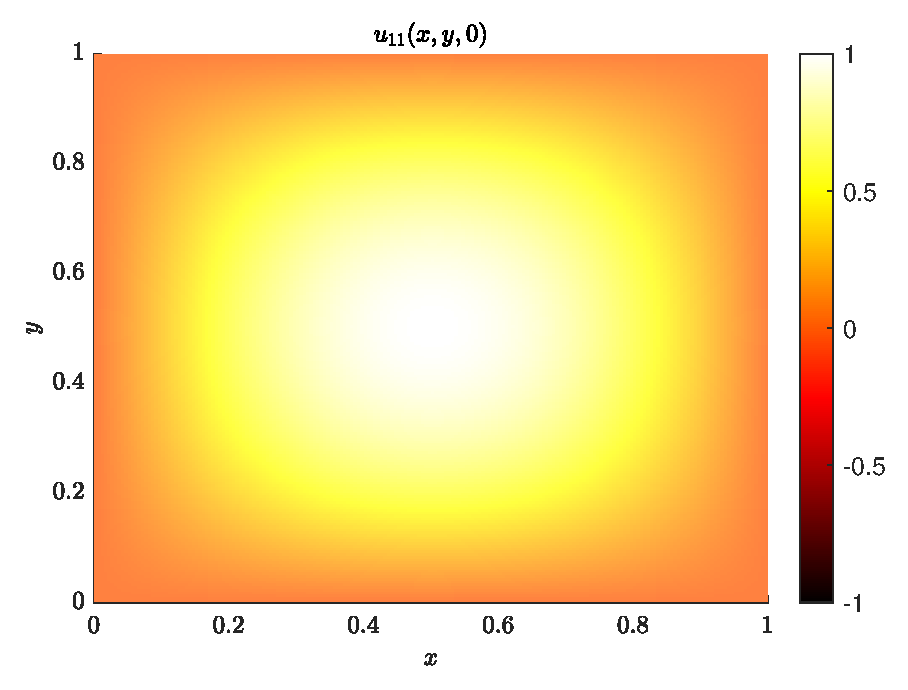
\includegraphics[width=\textwidth]{figures/heat_solution_t=0}
        \caption{Solution at $t=0$.}
        \end{subfigure}
\hfill
        \begin{subfigure}[b]{0.3\textwidth}
        	\centering
        	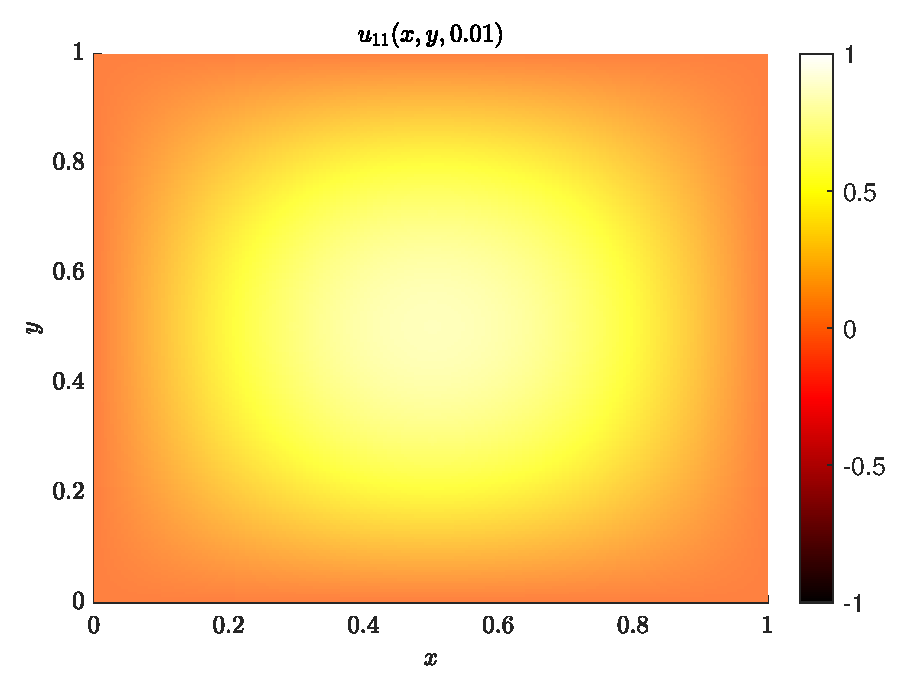
\includegraphics[width=\textwidth]{figures/heat_solution_t=0.01}
            \caption{Solution at $t=0.01$.}
        \end{subfigure}
\hfill
        \begin{subfigure}[b]{0.3\textwidth}
        	\centering
        	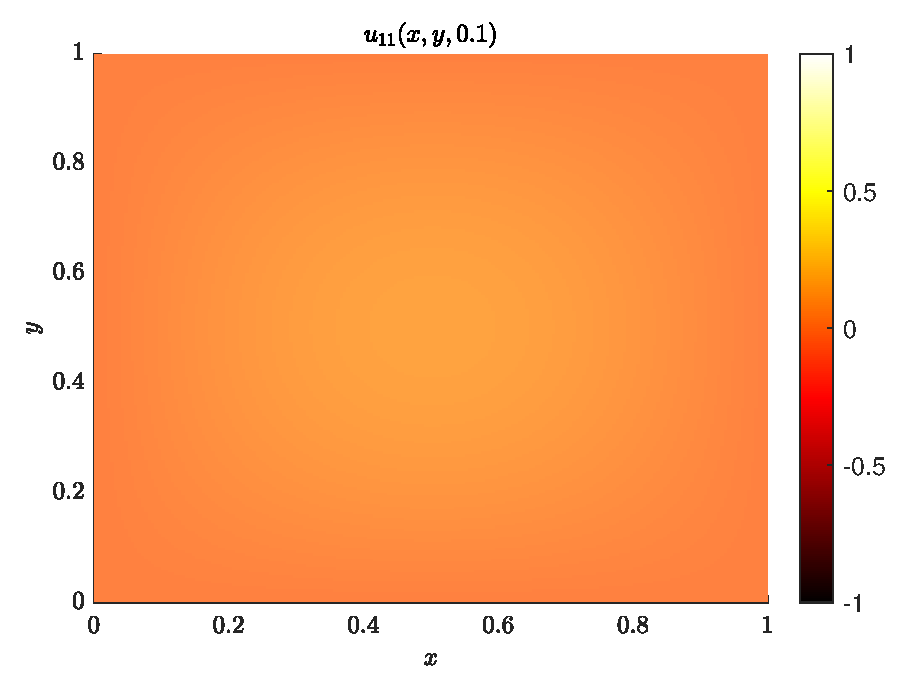
\includegraphics[width=\textwidth]{figures/heat_solution_t=0.1}
            \caption{Solution at $t=0.1$.}
        \end{subfigure}
\caption{The color displays the temperature as shown by the colorbar.}
\end{figure}
    As time moves forward, we find that the plate is cooling down to the temperature of the boundary.  So, the whole plate will reach a temperature of zero if we go indefinitely far in the future.
    
    \item $k$ decides how quickly heat will flow in our material. Larger values of $k$ means that temperature will flow more easily.  We can see this in the equation since a larger $k$ will make the exponential decay term in our equation approach zero more rapidly.  One can also repeat the plots in the previous part but for a larger value of $k$ to see this in action.
    
    \item The mathematical reason why is similar to what we discussed in the previous part.  If we increase $m$ or $n$, we find that the exponential decay happens at a quicker rate.
    
    \item Physically, as $m$ and $n$ increase, we have more hot and cold regions placed next to each other.  When there are two regions of vastly different temperature close to each other, they will equilibrate more quickly.  These two plots show what this looks like pictorially.
    \begin{figure}[H]
            \begin{subfigure}[b]{0.45\textwidth}
            	\centering
            	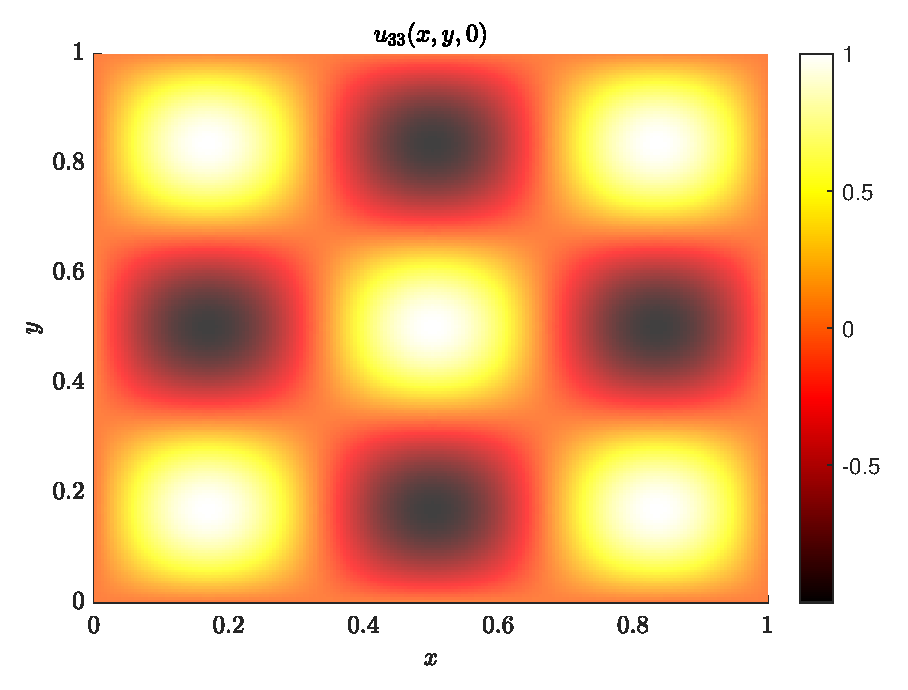
\includegraphics[width=\textwidth]{heat_solution_m=3_n=3}
                \caption{At $t=0$, this is the profile for $m=3$ and $n=3$.}
            \end{subfigure}
\hfill
            \begin{subfigure}[b]{0.45\textwidth}
            	\centering
                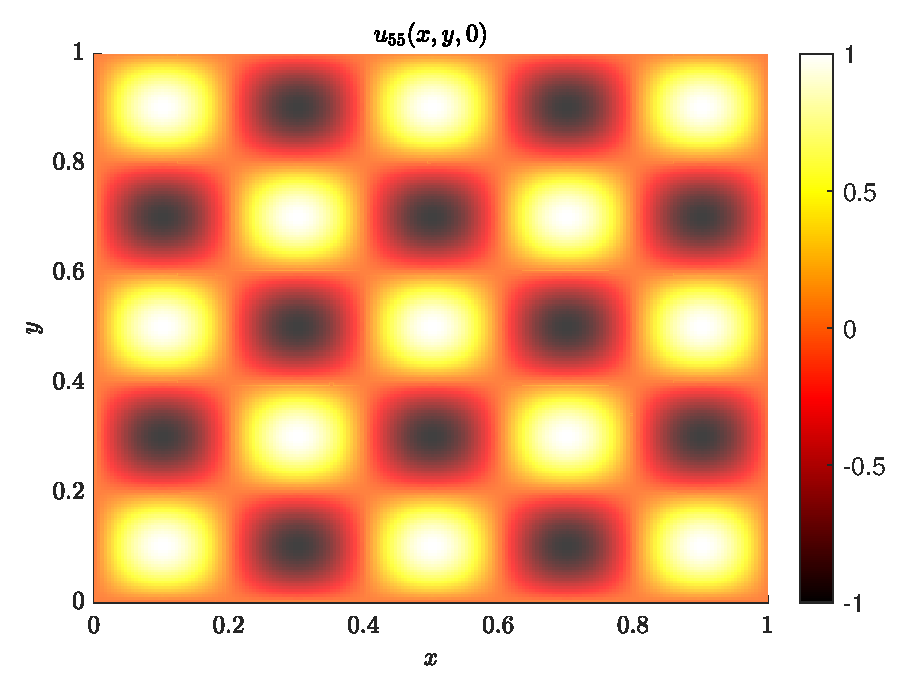
\includegraphics[width=\textwidth]{heat_solution_m=5_n=5}
                \caption{At $t=0$, this is the profile for $m=5$ and $n=5$.}
            \end{subfigure}
\caption{The color displays the temperature as shown by the colorbar.}
        \end{figure}
    
\end{enumerate}
\end{solution}

\end{document}